\documentclass[tikz,border=10pt]{standalone}
\usepackage{circuitikz}
\usepackage{xcolor}
\usepackage{amsmath}
\usetikzlibrary{arrows}

\begin{document}
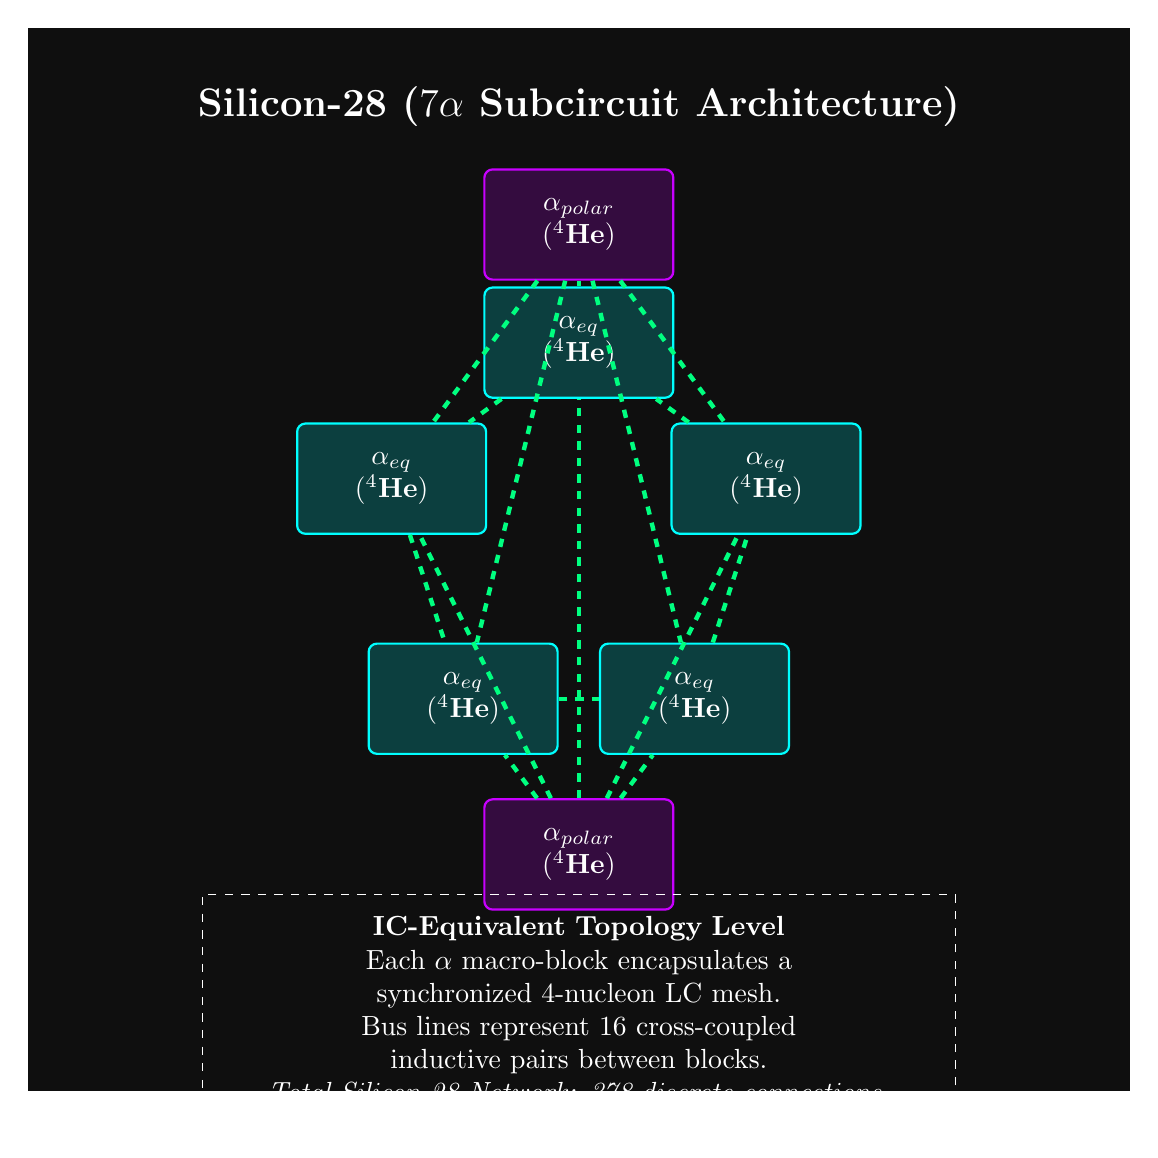
\begin{tikzpicture}[>=latex']

\definecolor{neonblue}{RGB}{0, 255, 255}
\definecolor{neongreen}{RGB}{0, 255, 128}
\definecolor{darkbg}{RGB}{15, 15, 15}
\definecolor{neonpurple}{RGB}{200, 0, 255}

% Fill background
\fill[darkbg] (-7,-7) rectangle (7,6.5);

% Title
\node[text=white, font=\bfseries\Large] at (0, 5.5) {Silicon-28 ($7\alpha$ Subcircuit Architecture)};

\tikzset{
    alpha block/.style={
        draw=#1, thick, fill=darkbg!80!#1,
        rectangle, rounded corners=3pt,
        minimum width=2.4cm, minimum height=1.4cm,
        text=white, font=\bfseries, align=center
    },
    bus/.style={
        draw=neongreen, ultra thick, dashed
    }
}

% EQUATORIAL PLANE (5 Alphas - Pentagon)
\node[alpha block=neonblue] (E1) at (90+72*0:2.5) {$\alpha_{eq}$\\$(^4\text{He})$};
\node[alpha block=neonblue] (E2) at (90+72*1:2.5) {$\alpha_{eq}$\\$(^4\text{He})$};
\node[alpha block=neonblue] (E3) at (90+72*2:2.5) {$\alpha_{eq}$\\$(^4\text{He})$};
\node[alpha block=neonblue] (E4) at (90+72*3:2.5) {$\alpha_{eq}$\\$(^4\text{He})$};
\node[alpha block=neonblue] (E5) at (90+72*4:2.5) {$\alpha_{eq}$\\$(^4\text{He})$};

% POLAR AXIS (2 Alphas)
\node[alpha block=neonpurple] (P1) at (0, 4.0) {$\alpha_{polar}$\\$(^4\text{He})$};
\node[alpha block=neonpurple] (P2) at (0, -4.0) {$\alpha_{polar}$\\$(^4\text{He})$};

% --- MACRO-COUPLINGS (BUS LINES) ---

% Equatorial Pentagon Ring
\draw[bus] (E1) -- (E2);
\draw[bus] (E2) -- (E3);
\draw[bus] (E3) -- (E4);
\draw[bus] (E4) -- (E5);
\draw[bus] (E5) -- (E1);

% Polar North to Equator
\draw[bus] (P1) -- (E1);
\draw[bus] (P1) -- (E2);
\draw[bus] (P1) -- (E3);
\draw[bus] (P1) -- (E4);
\draw[bus] (P1) -- (E5);

% Polar South to Equator
\draw[bus] (P2) -- (E1);
\draw[bus] (P2) -- (E2);
\draw[bus] (P2) -- (E3);
\draw[bus] (P2) -- (E4);
\draw[bus] (P2) -- (E5);

% Legend
\node[text=white, text width=9cm, align=center, draw=white, dashed, inner sep=8pt] at (0, -6) {
    \textbf{IC-Equivalent Topology Level}\\
    Each $\alpha$ macro-block encapsulates a synchronized 4-nucleon LC mesh.\\
    Bus lines represent 16 cross-coupled inductive pairs between blocks.\\
    \textit{Total Silicon-28 Network: 378 discrete connections.}
};

\end{tikzpicture}
\end{document}
